Hardware resource disaggregation is a new trend for building
datacenters as it solves several limitations of a traditional monolithic
server architecture~\cite{Intel_RSA, HP_The_Machine, FB_disaggregated_rack,
chung2018towards, katrinis2016rack, asanovic2014firebox,
lim2009disaggregated, shan2018legoos}. A traditional
monolithic architecture consists of a collection of server boxes, with
each box containing a collection of computer resources such as processors,
memory, NICs, and accelerators like GPUs.
In contrast, in a resource disaggregated datacenter computer resources
are partitioned into \emph{resource blades} connected by high performance
network switches.
Examples of resource blades include processor, memory, and
accelerator blades.
In a disaggregated datacenter there is no longer a
\emph{hard boundary} between different computers.
Instead, hypervisors and operating systems orchestrate
computer abstractions with \emph{soft boundaries}.

%-------------------------------------------------------------------------------
% Figure of the proposed architecture
\begin{figure}[]
     \centering
     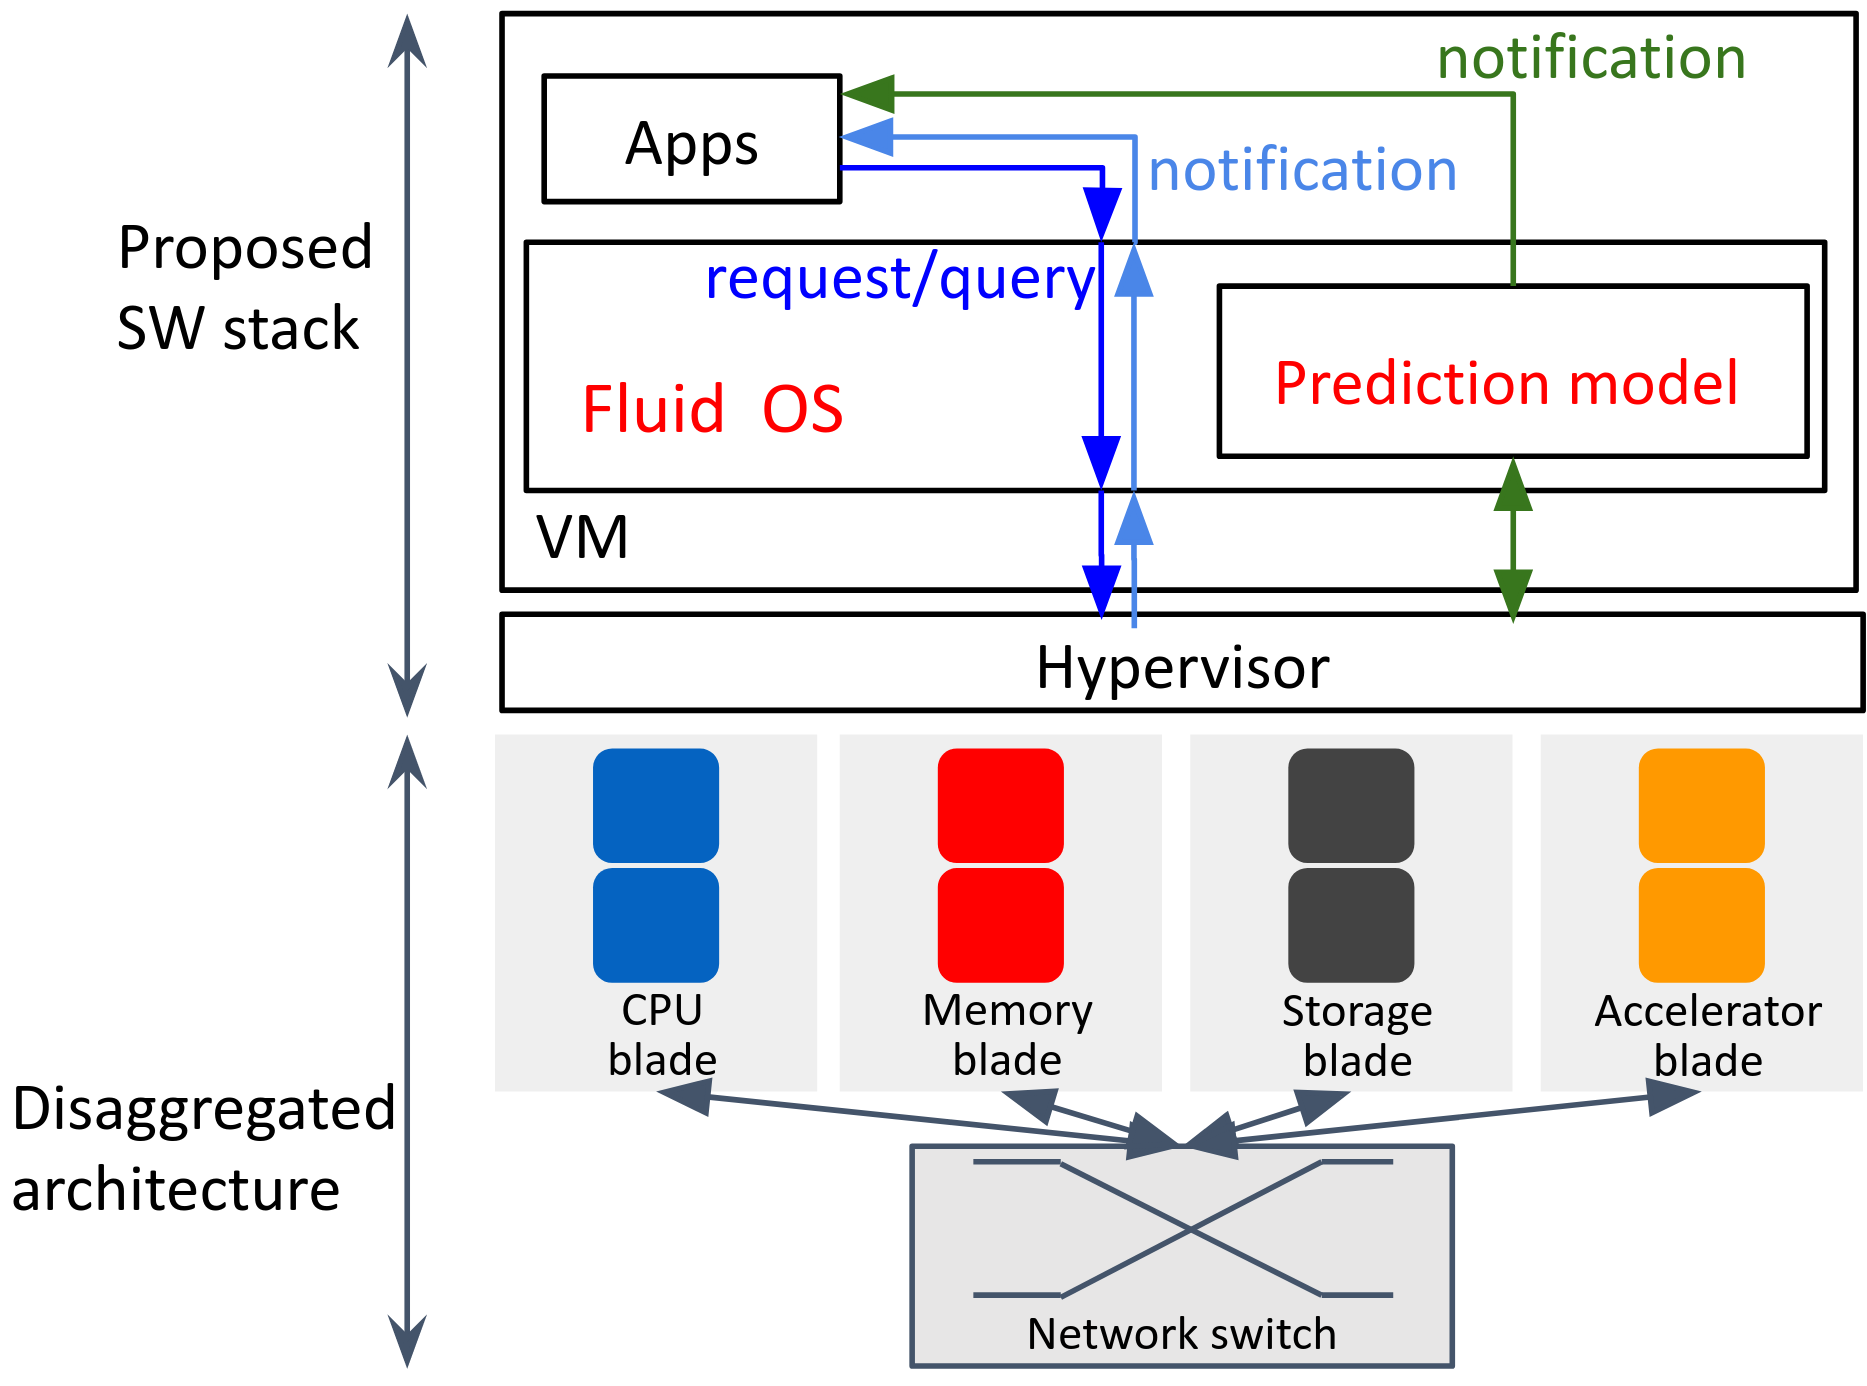
\includegraphics[scale=0.15]{images/architecture.png}
     \caption{Proposed architecture.}
     \label{fig:archi}
\end{figure}
%-------------------------------------------------------------------------------

Hardware resource disaggregation further realizes resource
elasticity~\cite{herbst2013elasticity} as computing resources can
be allocated across traditional server boundaries.  In a monolithic
architecture, the resources a virtual machine or container can
allocate are limited by the resources on the hosting physical
machine, while in a disaggregated architecture resources can be
allocated from much larger \emph{resource pools}.  Furthermore, in
a disaggregated architecture, each type of resource can be allocated
independently without considering the amount or availability of
other types of resources.  Because resource allocation is essentially
unbounded and independent, disaggregated architectures have the
potential to achieve better utilization than monolithic ones.

\begin{comment}
Take Amazon EC2~\cite{ec2} for example, the computing
resources of each EC2 instance type is pre-defined and fixed (e.g.,
m5.large type consist of 2 vcpu and 8 GIB memory).  This resource
relation constraint can no longer exist in a resource disaggregated
datacenter.
\end{comment}

To take full advantage of unbounded and independent resource
elasticity, we argue that operating systems running on the resource
disaggregated hardware should be \emph{continuously reconfigurable},
or, \emph{fluid}.
Here we define a \emph{fluid OS} to be an OS that allows
dynamically changing computing resources. For instance, an OS may
boot with 2 cores and 4 GB memory but it can allocate or deallocate
cores and memory according to its demands. Reconfigurability can
be further extended to storage devices, accelerators, NICs, and so
on.  Moreover, a fluid OS can also support dynamically
allocating different classes of the same computing resource (e.g.,
brawny vs.~wimpy cores for CPU, DRAM, 3D-stacked DRAM, NVM for
memory).
We also envision that a fluid OS provides new interfaces or
abstractions to its applications so they too can leverage the
disaggregated hardware architecture.

We target public cloud platforms where applications are
running in virtual machines. This assumption is realistic as most
of public cloud providers wrap users' software within virtual
machines.
Virtual machines simplify isolating tenants and allow
deployment of a variety of operating systems.
This concept also holds for containerized cloud and
serverless frameworks~\cite{agache2020firecracker}. As depicted in
Figure~\ref{fig:archi}, we assume there is a hypervisor running on
top of the disaggregated hardware and we can rely on it to manage
the underlying disaggregated hardware components. Moreover, this
hypervisor provides a new virtual machine abstraction consisting
of changing hardware resources instead of the fixed set of resources
available in a conventional virtual machine abstraction.

We are prototyping a fluid OS as a guest OS inside
a virtual machine. This allows us to focus on exploring the policies
and mechanisms required for supporting resource reconfiguration
without dealing with subtle hardware settings.
Section~\ref{sec:proposal} presents details about the
proposed architecture.

There are several benefits that can be obtained from
a fluid OS.
\begin{itemize}
\item The approach is optimal for memory-intensive applications as
memory can be allocated as needed.  A fluid OS is also
advantageous to memory-elastic applications~\cite{funaro2020memory}.
\item With the capability of allocating many cores and accelerators
in a single fluid OS, highly compute-intensive
workloads are more easily supported without the need to
explicitly distribute them across multiple machines.
\item A fluid OS supports heterogeneous resource usage,
like a workload allocating both brawny and wimpy cores and
different types of memory.
\item As resources can be requested unboundedly and independently,
the proposed architecture enables the Resource-as-a-Service
cloud cost model~\cite{ben2012resource}.
\end{itemize}

\begin{comment}
We elaborate the benefits more in Section~\ref{sec:benefits}. Beyond
that, we hope the support of resource reconfigurability can enable
a new programming paradigm and enlight more research directions.
\end{comment}

The paper is organized as follows.  Section~\ref{sec:background}
provides background and contrasts our proposed architecture with
prior work.  We motivate the fluid OS, elaborating on
benefits that can be obtained from the fluid OS in
Section~\ref{sec:fluid_os}.  We present challenges and research
opportunities in Section~\ref{sec:opportunities}.
Section~\ref{sec:proposal} provides details of our proposed
architecture and in particular the fluid OS.
Section~\ref{sec:conclusion} concludes.
